

\fancypagestyle{miEstilo3}{
   \lhead{3. Análisis de mercado}
   %\chead{1. Introducción}
   \rhead{Página \thepage}
   \lfoot{}
   \cfoot{}
   \rfoot{}
}

\pagestyle{miEstilo3}

\section{Análisis de mercado}

Antes de comenzar con el desarrollo del proyecto, se ha realizado un estudio de mercado para comprobar si hay algún tipo de sistema similar ya implementado, qué características tiene, y qué posibles diferencias habría con el que se tiene pensado implementar.

Es cierto que la raspberry PI tiene infinidades de posibles aplicaciones, y que en la web se puede encontrar todo tipo de tutoriales e ideas para poder explotar al máximo su uso, pero ¿existirá algún tipo de sistema de seguridad que sea funcional, fácil de instalar y utilizar?. Para responder a esta pregunta, se ha realizado una búsqueda intensiva en la web y youtube, ya que suelen ser los principales medios donde se publica este tipo de información.

Investigando, se ha descubierto que hay múltiples páginas y vídeos que hacen referencia al uso de una raspberry PI con una cámara, y su posible aplicación para poder visualizar en tiempo real la grabación realizada por la cámara.

A continuación se van a detallar los principales aspectos a destacar de los sistemas encontrados.

\subsection{Proyecto: Build a Raspberry Pi Security Camera Network} \label{sec:pj1}

Este es un proyecto \cite{ref2} que se basa en el uso de una distribución Linux llamada \texttt{motionEyeOS} y de código abierto \cite{ref3} que convierte una raspberry PI en un sistema de videovigilancia.

Si leemos la descripción de este proyecto \cite{ref2}, podemos observar como se hace una pequeña descripción de los componentes necesarios y una guía de instalación del sistema \texttt{motionEyeOS}.

Entre sus principales características, podemos encontrar las siguientes:

\vspace{-0.5cm}

\begin{itemize}
\item \textbf{Acceso restringido}: Consta de unas credenciales (usuario y contraseña) para poder acceder a la visualización y configuración de las cámaras.

\item \textbf{Sistema multicámara}: Es un sistema que soporta la visualización e interacción con múltiples cámaras simultáneamente conectadas en la misma red.

\begin{figure}[h]
	\centering
	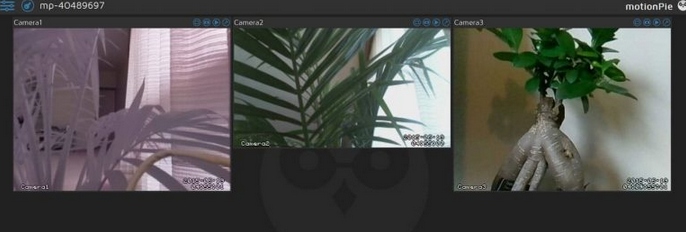
\includegraphics[scale=0.4]{images/1}
	\label{imagen2}
	\caption{Sistema de seguridad con 3 cámaras}
\end{figure}

\item \textbf{Conexión via wifi}: Este sistema soporta la conexión via wifi. Será necesario añadir el SSID y clave de la red.

\item \textbf{Configuración de la cámara}: El sistema consta de un menú para poder configurar la cámara. Los parámetros configurables son:

	\begin{itemize}
	\item Nombre de la cámara: Nombre para poder identificar la cámara.
	\item Filtrado de luz: Filtro para evitar falsos positivos ante el encendido y apagado de una luz.
	\item Brillo automático: Configuración automática de brillo y contraste de luz.
	\item Resolución de la cámara: Configuración para poder modificar la resolución de la cámara.
	\item Rotación de la cámara: Rotación de la imagen de vídeo o cámara.
	\item FPS: Configuración del número de frames por segundo (imágenes por segundo).
	\end{itemize}

\item \textbf{Almacenamiento}: Es posible almacenar los archivos de imagen o vídeo.

\item \textbf{Fecha y hora}: Posibilita la opción de mostrar fecha y hora durente la grabación de un vídeo o la captura de una foto.

\item \textbf{Vídeo streaming}: Permite la visualización del vídeo capturada por las cámaras en tiempo real.

\item \textbf{Detección de movimiento}: El sistema permite la detección de movimiento y en consecuencia la grabación de un vídeo o la captura de una foto.

\item \textbf{Alertas}: Es posible generar alertas via email o webhook cuando se detecta movimiento.

\end{itemize}

\subsection{Proyecto: Raspberry Pi As Low-cost HD Surveillance Camera}\label{sec:pj2}

Este es un proyecto \cite{ref4} bastante simple y centrado en la vigilancia el cual está basado en \texttt{Motion detection software} \cite{ref5}. Este es un software de código abierto y disponible en los repositorios de raspbian para poder monitorizar las señales de vídeo para varios tipos de cámaras (entre ellas la PiCamera).

Algunas de las características de este software son:

\vspace{-0.5cm}

\begin{itemize}
\item Grabación de vídeos y/o capturas de fotos.
\item Visualización de vídeo en tiempo real (streaming).
\item Gestión de actividades y activación de scripts tras dichos eventos.
\item Registro de eventos en bases de datos.
\item Plantillas personalizables para detección de movimiento.
\item Soporte completo de TLS (https) con autenticación y control web para streaming.

\end{itemize}

En este proyecto, se hace una descripción de los componentes necesarios para poder montar este sistema, e incluso se hace una estimación del precio de dichos componentes y se proporciona un enlace de compra.

A continuación se proporciona una guía básica de instalación y configuración, mostrando los siguientes resultados:

\newpage

\begin{figure}[H]
	\centering
	\begin{subfigure}[b]{0.3\textwidth}
		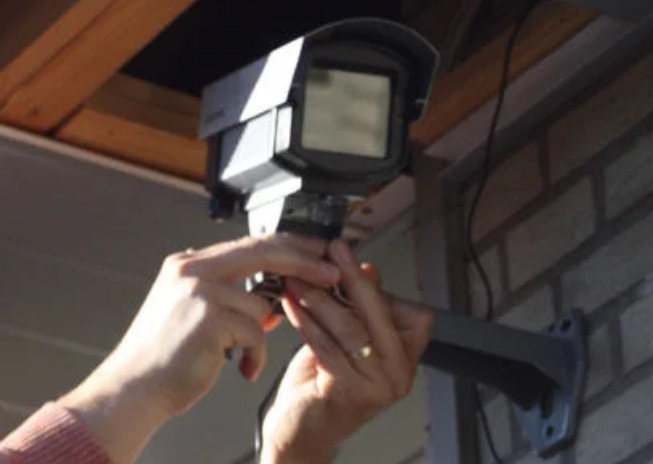
\includegraphics[width=\textwidth,height=90px]{images/2}
		\caption{Colocación de la cámara}
	\end{subfigure}
	~ 
	\begin{subfigure}[b]{0.3\textwidth}
		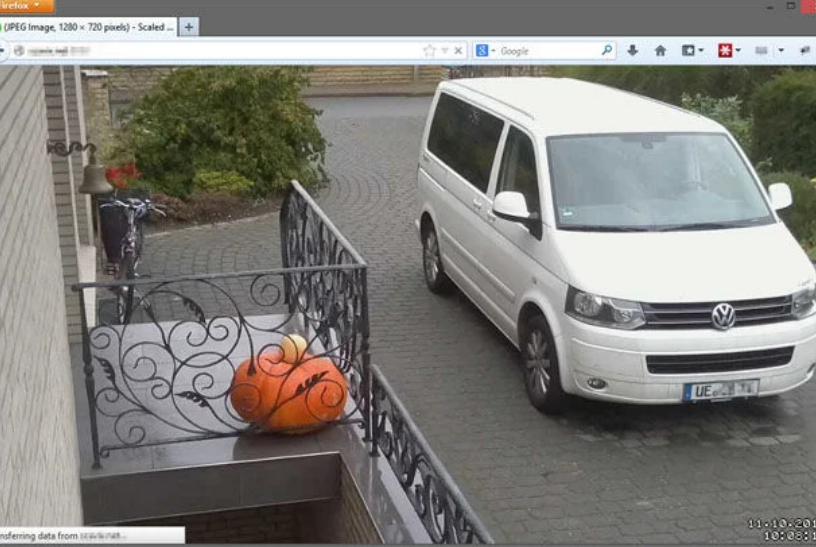
\includegraphics[width=\textwidth,height=90px]{images/3}
		\caption{Streaming}
	\end{subfigure}
	\caption{Sistema de videovigilancia}

\end{figure}

\subsection{Proyecto: sensor de movimiento y cámara con envío de imágenes a correo} \label{sec:pj3}

Este es un proyecto descrito en un vídeo de youtube \cite{ref6} que explica cómo construir un pequeño sistema de seguridad basado en la detección de movimiento, captura de una foto y envío de la foto capturada tras haberse activado la detección de movimiento.

En este vídeo se explica qué componentes son necesarios, cómo conectarlos y se proporciona un script de Python que se encarga de la detección de movimiento y envío de la imagen al correo gmail, utilizando librerías de Python como \textit{PiCamera} y \textit{smtplib}.

Este proyecto no tiene complejidad alguna, ya que es muy simple y todo está explicado para cualquier usuario, además de ser un buen comienzo para empezar a investigar y probar el mundo de la videovigilancia basada en bajo coste.

\subsection{Conclusión}

Investigando por la web, he descubierto que hay muchos tipos de proyectos similares a los mencionados, unos más simples y otros más complejos, pero en general todos comparten el objetivo de poder vigilar una zona a través de una cámara y una raspberry PI.

\newpage

Otro de los principales aspectos a destacar, es que la mayoría hacen el uso del software libre \texttt{motionEyeOS} o \texttt{motion agent detection} que se han mencionado en las secciones \ref{sec:pj1} y \ref{sec:pj2}.

El objetivo de este proyecto no es 'volver a reinventar la rueda` sino hacer de este un proyecto innovador y con un valor añadido respecto al resto.

Por ello, se ha diseñado y propuesto un sistema que cumpla con la mayoría de características de proyectos similares, combinando lo mejor de cada uno, y añadiendo nuevas funcionalidades adicionales que hagan que sea una de las mejores opciones a la hora de plantearse implementar un sistema de videovigilancia de bajo coste.

Según he podido observar, hay muchos proyectos en los que la documentación es escasa y no muy concisa, además de realizar instalaciones y configuraciones a bajo nivel. Esto hace que cualquier usuario no tenga acceso a este tipo de aplicaciones, ya que requieren un usuario medio-avanzado en conocimientos informáticos.

Por ello, se ha tenido en cuenta la simplicidad del software y su fácil gestión y uso, además de intentar cubrir todos los principales aspectos de una videovigilancia.

En las siguientes secciones, se mostrará más en detalle qué funcionalidades tiene esta aplicación, pero para mostrar sus principales aspectos clave y diferenciadores respecto al resto se va a realizar una comparación, tal y como se puede observar en la siguiente tabla.


Observando la tabla \ref{table:1}, se puede comprobar como la aplicación propuesta cumple con la mayoría de las características del resto de proyectos actuales, y mejora en otros aspectos.

Como aspecto a destacar, decir que el proyecto propuesto consta de una aplicación backend y una aplicación multiplataforma de usuario, además de ser fácil uso y estar documentada. Estos aspectos principales aportan una gran versatilidad a este proyecto, siendo sin duda la mejor opción hasta el momento desarrollada en el ámbito de la videovigilancia de raspberry PI.

También, como trabajos futuros, se desea implementar la funcionalidad multicámara, haciendo posible la interacción con más de una cámara simultáneamente.

\newpage

\begin{table}[h!]
\centering
\begin{tabular}{|l|c|c|c|c|}
\hline
\rowcolor[HTML]{EFEFEF} 
 \textbf{ Proyectos} & \hyperref[sec:pj1]{Proyecto 1}  & \hyperref[sec:pj2]{Proyecto 2} & \hyperref[sec:pj3]{Proyecto 3} & SIVIRA \\ \hline
Captura de imagen & \cmark & \cmark  & \cmark & \cmark \\ \hline
\rowcolor[HTML]{fcfcfc} 
Grabación de vídeo & \cmark  & \cmark  & \xmark & \cmark \\ \hline
Streaming & \cmark  & \cmark & \xmark & \cmark \\ \hline
\rowcolor[HTML]{fcfcfc} 
Alertas & \cmark  & \cmark & \cmark & \cmark \\ \hline
Filtrado de alertas inteligente & \xmark   & \xmark & \xmark & \cmark \\ \hline
\rowcolor[HTML]{fcfcfc} 
Aplicación de usuario & \xmark & \xmark & \xmark & \cmark \\ \hline
Soporte multicámara & \cmark  & \cmark & \xmark & \xmark \\ \hline
\rowcolor[HTML]{fcfcfc} 
Fácil instalación y uso & \xmark  & \xmark & \cmark & \cmark \\ \hline
Cámara configurable & \cmark  & \xmark & \xmark & \cmark \\ \hline
\rowcolor[HTML]{fcfcfc} 
Documentación & \xmark & \xmark & \xmark & \cmark \\ \hline
Almacenamiento de eventos & \xmark  & \cmark & \xmark & \cmark \\ \hline
\end{tabular}
\caption{Comparativa de los distintos proyecto}
\label{table:1}
\end{table}

\color{black}
